%===================================== CHAP 3 =================================

\chapter{Related Work}
\label{chap:relatedWork}
The recent advancement in virtual, augmented and mixed reality (VR/AR/MR) technologies by companies such as Oculus and Microsoft 
has contributed to the development of applications which aims to solve real world problems. The field of Computer Supported Collaborative Learning (CSCL) (see Section \ref{section:CSCL}) and Computer Supported Cooperative Work (CSCW) has according to Ens et al. over the last three decades culminated in rich theory about collaboration and how it can be more than just the sum of its parts \cite{ens2019revisiting}.

Although the use of VR/AR/MR for collaborative tasks has been studied considerably over the years, not much research has gone in the field of using VR, collaboration, design principles and tools for developing and evaluating collaborative virtual internship and experiences. 

\subsubsection{Inclusion Criteria}
\label{section:inclusionCriteria}
For related work to be eligible to included in this thesis there are elements that must be present in the research paper for it to selected. These characteristics are used as inclusion criteria in order to adjust scope of the search for related work. These are listed below:

\begin{itemize}
\label{itm:inclusionCriteria}
\setlength\itemsep{0em}
  \item Date of publication. Must have been published in 2014 or later.
  \item Language of publication. Must be in English or Norwegian.
  \item Must include virtual reality (VR).
  \item Must include either collaboration aspect or teaching/workplace training aspect.
\end{itemize}


This chapter will review and discuss related work and then compare their respective features that are relevant for this thesis. 




\section{Virtual Workplace Internship Using Virtual Reality}
\label{section:VRworkplaceIntership}
The IMTEL lab (see Section \ref{section:context}) is researching an ongoing project called \textit{virtual internships} which aims to help young job seekers getting insight into various professions including road construction and fishery worker using virtual reality. Prasolova-Førland et al. \cite{prasolova2019empowering} published a paper in 2019 detailing the results of their developed concept \textit{immersive job taste}, an immersive and interactive experience in regards to the virtual internship project at IMTEL. The paper evaluated different virtual and augmented reality prototypes (including the "Fishery VR" application) and found that results indicate a generally positive attitude towards the concept of immersive job taste \cite{prasolova2019empowering}. The idea of the prototypes is to provide the feeling and interactive experience of a real world workplace with basic training and introduction of its everyday tasks. This is illustrated in Figure \ref{fig:FisheryVR} showcasing some of the virtual workplace internship tasks and experiences available in the FisheryVR application, including fillet cutting and boat driving. 

 \begin{figure}[!ht]
     \centering
     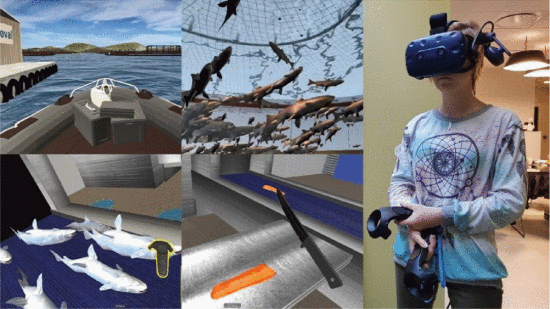
\includegraphics[width=.7\textwidth]{./fig/related_work/fisheryVR.png}
     \caption{FisheryVR screenshots (left) and the user (right) \cite{prasolova2019empowering}.}
     \label{fig:FisheryVR}
 \end{figure}

Prasolova-Førland et al. \cite{prasolova2019empowering} states that it can provide a low-threshold alternative or supplement internships using innovative technologies with gaming elements. Gamification for training and educational purposes is a supported method as concluded by Hamari et al. \cite{hamari2014does}. These virtual reality applications allows young job seekers to gain interest and understanding about the workplace which was evident by the project test participants as they found them to be enjoyable and engaging. 

However, there are several aspects to consider when using virtual reality as a immersive tool for workplace experience. This includes the importance of feedback, engagement and self-efficacy. According to Prasolova-Førland et al. (\citeyear{prasolova2019empowering}) the literature and results indicate that more feedback in the application is needed for a higher educational experience. They suggested NPCs (non-playable characters) in different roles, e.g. colleagues. This can be transferable to our project, but instead of utilising NPCs we can embed multi-user functionality. This enables participation of career counsellors, other peers and industry representatives in the same simulation which might increase engagement and realism. It also opens up for collaboration amongst players and as the paper describes the typical self-efficacy amongst the target group (i.e. young job seekers) is low, but perhaps with collaboration opportunities and feedback this can have an positive impact and contribute to the learning efficacy.  



\section{ElectroVR: Collaborative Learning in Virtual Reality}
\label{section:electroVR}
In 2019 Greenwald et al. published a paper were they presented ElectroVR, an playground for collaborative simulation-based exploratory learning using virtual reality \cite{greenwald2019electrovr}. The project presents a demo application combining three learning approaches including embodied learning in immersive six-degree-of-freedom (6DoF)  VR,  simulation-based  exploratory  learning,  and collaborative learning. The system allows two co-located users using HTC Vive as HMDs to explore and interact with the environment which is based electricity and  magnetism simulations, see Figure \ref{fig:electroVR}.

 \begin{figure}[!ht]
     \centering
     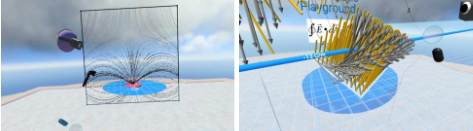
\includegraphics[width=.9\textwidth]{./fig/related_work/electroVR.PNG}
     \caption{ElectroVR in use with visualisations and avatar representation (left) \cite{greenwald2019electrovr}. }
     \label{fig:electroVR}
 \end{figure}
 
Greenwald et al. (\citeyear{greenwald2019electrovr}) convey that the system shows off co-located, multi-user tracked virtual reality and a playback system for narrative sequences prepared by instructors. The system can therefore support the use of only peers (learners) or a more instruction focused use with a single peer and instructor. They use a client server architecture to allow for synchronisation of interactive objects such as tools or avatars. The avatars are simple representations of the users with corresponding movement which according to  Greenwald et al. \cite{greenwald2017investigating} yields a strong a sense of social presence and is effective for gesture based communication. There is also narrator functionality allowing recordings of sound to be played back to learners as part of the instructions, but there are no real-time voice chat.

Noticeably the system is built on previous work and integration done by the same author in 2017 where they described \textit{"CocoVerse"}, a shared co-located virtual environment for collaboration \cite{greenwald2017multi}. The paper lacks adequate data results and analysis and cannot therefore a this point of time conclude with any legitimate findings based on the system. They do however emphasise that this is a ongoing project and that initial testing by students have given positive feedback. The future of this project will investigate the effectiveness of collaborative learning in virtual reality through rigorous testing \cite{greenwald2019electrovr}.  





\section{CoVAR: Virtual and Augmented System for Remote Collaboration}
\label{sec:coVAR}
In 2017 Piumsomboon et al. published a paper presenting a remote collaboration system combining augmented reality, virtual reality, and natural communication to create new types of collaboration \cite{piumsomboon2017covar}. Named \textit{CoVAR}, the system aims to combine the best of both VR and AR and use their respecting strengths by reconstructing the environment seen by the user who is wearing AR headset (Microsoft HoloLens) and displaying it to the VR user (using HTC Vive) so that they both share the same view, see Figure \ref{fig:coVAR}. Thus enabling collaboration for the use of observing 3D objects, experience scenes/environments or other. Remote collaboration is achieved by using an client server architecture where data synchronisation is handled by Unity networking, UNet (which at the point of writing this thesis is deprecated) \footnote{https://support.unity3d.com/hc/en-us/articles/360001252086-UNet-Deprecation-FAQ}.


\begin{figure}[!ht]
     \centering
     \includegraphics[width=.9\textwidth]{./fig/related_work/coVAR.png}
     \captionsetup{width=0.9\linewidth}
     \caption{CoVAR in use with reconstrucuted enviroment (A left) and AR user (B left) and VR user (B right) looking at a block object.  \cite{greenwald2019electrovr}. }
     \label{fig:coVAR}
 \end{figure}

The system has various interaction methods, virtual awareness cues and view enhancement to support and enhance collaboration. Interaction methods includes hand gestures, head gaze, and eye gaze input. The paper describes collaborative gaze as a technique where users gaze at the same target object to trigger an action such as revealing hidden information \cite{piumsomboon2017covar}.  Virtual awareness cues includes methods as a ray showing the users eye direction. View enhancement techniques includes features like "god" or "miniature" mode and snapping the VR user to the AR users head placement.

This system is intriguing as it provides a new approach to collaborative VR and AR, combining both of them. The gazing technique is interesting for collaboration as it illustrates interest in objects and according to Piumsomboon et al. (\citeyear{piumsomboon2017covar}) allows the VR user to know exactly where the AR user is and what they were looking at. However, CoVAR supports remote collaboration but does not implement voice communication solely relying on gestures and gazing which can be potentially be challenging for the users.   



% \section{Archaeological excavation}
% In 2004 Benko et al. published a paper were they presented VITA (visual interaction tool for archaeology) an experimental collaborative mixed reality system for offsite visualisation of an archaeological dig \cite{benko2004collaborative}. The system allowed multiple archaeologists to collaborate remotely using several interaction methods including gestures to manipulate and explore a real life terrain model, see Figure \ref{fig:VITA}. The system utilised see-through HMDs (augmented reality headset) and a high resolution screen to visualise the archaeological dig sites, a fairly complex system architecture with several components. To facility collaboration between the users of the system used voice commands and hand gestures. The paper evaluated the user experience using experts in the archaeological field, stating the initial user reactions were very positive \cite{benko2004collaborative}.

% However, before evaluation began participants where given an hour-long introduction and they were accompanied with an developer during the testing. This is not suitable or practical for the primary users for this thesis as the there are limitations in regards to time and other factors in regards to introduction of the application. The application should not require expert knowledge as a young job seeker or long introduction to its usage, but be intuitive and easily interpretable. Also, a critique from their system was that collaborating users should know were other users are looking.
% Benko et al. explored the possibility of the VITA system to be used a learning tool and the outcome was promising as users gained deeper understanding of archaeological sites. This is very transferable to the ongoing NAV workplace projects - aiming to let young job seekers understand and be introduced different workplaces remotely.      

% \begin{figure}[!h]
%     \centering
%     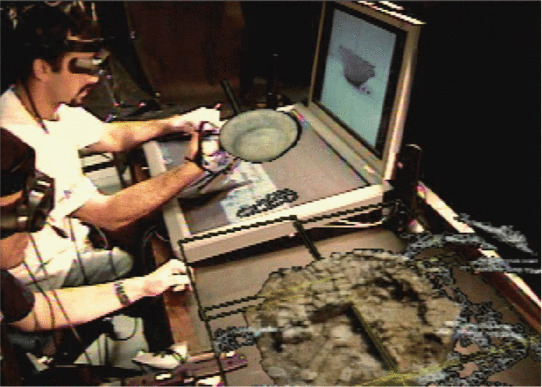
\includegraphics[width=.7\textwidth]{./fig/related_work/VITA.jpeg}
%     \caption{Two users simultaneously collaborate in VITA. \cite{benko2004collaborative}}
%     \label{fig:VITA}
% \end{figure}


\section{Mixed-reality to support co-creative collaboration}
Gardner and Sheaffer (\citeyear{gardner2017systems}) examines and discusses in Chapter 9 of the \textit{Virtual, Augmented, and Mixed Realities in Education} \cite{liu2017virtual} book, the use of mixed-reality in education and learning. Their work is focused around collaborative perspective with the \textit{MiRTLE} platform (Mixed Reality Teaching and Learning Environment) as their platform base.    
As Gardner and Sheaffer points out, the concepts \textit{immersion}, \textit{presence} and \textit{engagement} are important for the use of VR in education. In a multi-user environment the concepts can all contribute to an improved feeling of achievement for the participants within such multi-user virtual spaces \cite{gardner2017systems}. As such, they developed the MiRTLE system, a mix between video stream and virtual reality with the aim of being used in classrooms for educational proposes to support co-creative collaborative learning environments. In the paper it is described that the MiRTLE was extended by other institutions and universities, such as the \textit{BReal Lab} application (see Figure \ref{fig:BReal}) which provides geographically distributed learners to collaborate around physical engineering \cite{gardner2017systems}. It is a mixed-reality environment maker space. The testing of BReal Lab application showed a positive effect for learners experience and that it has potential for online education.            

\begin{figure}[!ht]
     \centering
     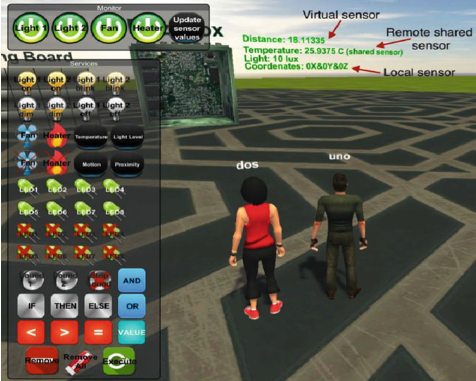
\includegraphics[width=.7\textwidth]{./fig/related_work/BReal.PNG}
     \captionsetup{width=0.6\linewidth}
     \caption{Screenshot of the BReal Lab application, a mixed-reality maker space for collaboration.}
     \label{fig:BReal}
 \end{figure}
 
 
 Although the tests of the different systems (MiRTLE, BReal Lab etc.) are generally positive and show  potential, there are also challenges for designing and making such co-creative collaborative spaces. According to Gardner and Sheaffer making them effective can both be demanding and time consuming, requiring high technical knowledge to include a high degree of immersion to increase the user experience \cite{gardner2017systems}. In other words, virtual and mixed-reality worlds are exciting and have great potential, but can struggle to compete with the real world in terms of immersion, presence and experience.          


\section{Virtual Reality Job Interview Training}
Smith et al. describes in their 2014 paper a developed prototype called \textit{VR-JIT}, a virtual reality job interview training system \cite{smith2014virtual}. The system was aimed at training adults with autism spectrum disorder for job interviews. Through randomised testing they measured both the feasibility and efficacy of the VR-JIT system where adults with autism participated in simulated job interviews with virtual characters using speech recognition software. Figure \ref{fig:vr-jit} shows the VR-JIT system in action with the interactive virtual character which is part of the interview training.   


\begin{figure}[!ht]
     \centering
     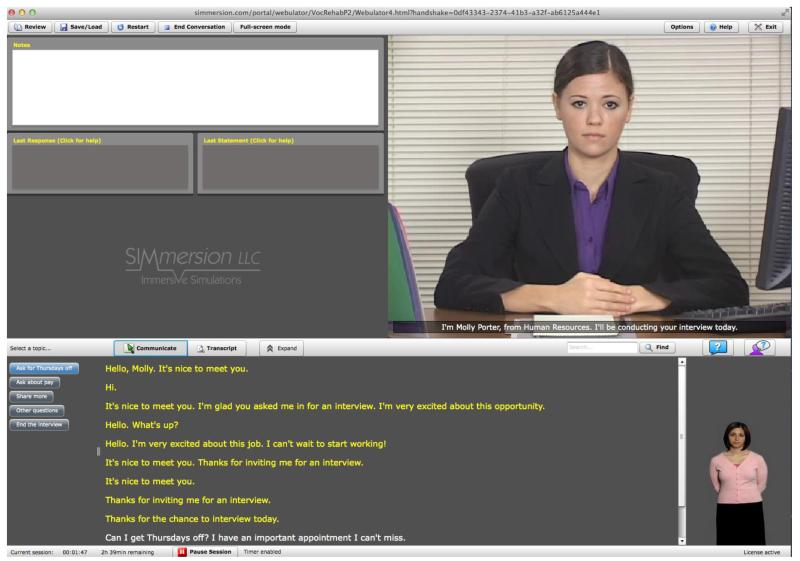
\includegraphics[width=.7\textwidth]{fig/related_work/vr-jit.jpg}
     \captionsetup{width=0.7\linewidth}
     \caption{The VR-JIT system.}
     \label{fig:vr-jit}
 \end{figure}
 
Testing was done with two groups, one using VR-JIT and the other using treatment as usual. According to the results, participants who used VR-JIT had greater improvement during live interviews and was reported to have higher self-confidence. Smith et al. found indications that the VR-JIT system is feasible and efficacious  to enhance practical job interview skills for adults with autism \cite{smith2014virtual}. The study was however limited in scope and resources, but it provides support that VR can be used effectively for virtual workplace training.  



\section{Other considerations}
As described in the beginning of this chapter  we presented inclusion criteria (see list \ref{itm:inclusionCriteria}) for related work. There are however some research papers which fall short of these but contribute with interesting and noteworthy features. These will be presented in this section.     

\subsection{Collaborative Virtual Reality Neurosurgical Training}
A 2007 paper by Kockro et al. describes their attempt at making a collaborative virtual reality environment for planning and training for neurosurgery \cite{kockro2007collaborative}. This came at a time where HMDs were less accessible, so the technology is not quite the same as is used now, but still falls within the MR spectrum. This project uses an interactive console with hand- and device-tracking that allows for manipulation of 3D data. This data is then displayed with a stereoscopic projector to the rest of the team so the collaboration can take place.

Perhaps the most interesting part is that they mention they underestimated the importance of collaboration for learning, stating that "\textit{...collaboration is more important than we imagined, and that the mutual exchange of individual concepts and ideas is a real benefit...}" \cite{kockro2007collaborative}. A previous attempt had been made without the collaborative aspect, but had not achieved the same results. This lends some credence to our initial hypothesis that the efficacy of the NAV applications could be improved were multi user functionality to be introduced. 

\subsection{Language Teaching in Virtual Reality}
The IMTEL lab has produced several master theses in relation to VR applications. One thesis by  Morte and Skjæveland \cite{morte2019effects} is not relevant in regards to workplace internship, but their application has features which can be beneficial for this project. The project focused on language teaching using collaborative techniques to help immigrants learn Norwegian. While their focus was on language teaching, there are still some valuable experiences to learn from, particularly when it came to the technical implementation including voice-chat and their networked multiplayer framework utilisation. Morte and Skjæveland (\citeyear{morte2019effects}) found that distributed collaboration has potential and that the increased presence affects the motivation of the users. Their application also included the option of having symmetric or asymmetric roles for its users, meaning one can be a student and student or student and teacher displayed as avatars in the VR environment. This can be transferred to our projects where we would have the possibility to be either a job seeker or a supervisor/mentor in the workplace training environment.     

\section{Comparison of related work}
\label{section:comparisonRelatedWork}
Table \ref{table:comparisonRelatedWork} provides an overview of the relevant features the different related work have. The comparison includes features which we have identified as important for this thesis by studying previous related applications and existing research in the field. As evident by the table, there are gaps in the field of research. 
There exists systems with collaboration and workplace training or guidance, but few combine both. Previous research done by the IMTEL lab shows there is a lack of this combination, and the need is further strengthened by users as the most request feature from a report summarising the results \cite{NavVRrapport}.       



An application has the features if it uses virtual reality, has multiplayer functionality (networked connection), includes workplace training, allows for collaboration, provides real world simulations (e.g. changing a tire), allow users to talk and hear each other using microphones and speakers, users are situated in the same space (co-located) or provides functionality for remote use (users not in the same space) and it allows for users to have the same role (symmetric role) or asymmetric roles such as peer and instructor.         
It is intended to summarise the the superficial aspects of the works, and act as a guide as to where one can find information about different implementations of a feature or combination thereof, e.g. multiplayer and VR or remote workplace training.  
\\
\newcommand*\ON[0]{$\surd$}
\newcommand*\LIM[0]{$\div$}
\\ "\ON" = has the feature.
\\ "\LIM" = has the feature, but is limited.

\begin{table}[!ht]
    \begin{center}
    \begin{tabular}{@{}l c c c c c @{}}
           & \multicolumn{5}{c}{\textbf{Related Work}}
    \\  \cmidrule{2-6}
           & \textbf{Workplace}
    \\       
             \textbf{Features}
           & \textbf{Internship}
           & \textbf{ElectroVR}
           & \textbf{CoVAR}
           & \textbf{BReal Lab}
           & \textbf{VR-JIT}
    \\ \midrule
       VR                           & \ON & \ON  & \ON  &  & \ON
    \\ Multiplayer                  &     & \LIM & \LIM & \ON &
    \\ Workplace training           & \ON &      &      &  & \ON
    \\ Collaboration                &     & \ON  &      & \ON & 
    \\ Real-world simulation        & \ON & \LIM & \ON  & \LIM & \ON
    \\ Voice-chat                   &     &      &      &  & 
    \\ Co-located                   & \ON & \ON  & \LIM &  &
    \\ Remote                       &     &      & \ON  & \ON &    
    \\ Symmetric role               & \ON & \ON  & \LIM & \ON  &
    \\ Asymmetric role              &     & \ON  & \LIM  & & \ON
    \\ \bottomrule
    \end{tabular}
    \captionsetup{width=1\linewidth}
    \caption{Comparison of applications, and relevant features for each of them.}
    \label{table:comparisonRelatedWork}
    \end{center}
\end{table}







\cleardoublepage